\documentclass{paper}
\usepackage[utf8]{inputenc}

\usepackage[version=4]{mhchem}
\usepackage{siunitx}
\usepackage{longtable,tabularx}
\setlength\LTleft{0pt}

\usepackage{hyperref}
\hypersetup{
    colorlinks,
    citecolor=black,
    filecolor=black,
    linkcolor=black,
    urlcolor=black
}
\usepackage{enumitem}
\usepackage{booktabs}
\usepackage{graphicx}
\usepackage{subcaption}
\usepackage{amsmath}
\usepackage{setspace}
\usepackage{amsmath}
\usepackage{tikz}
\usetikzlibrary{arrows}
\usepackage{color}
\usepackage{flexisym}
% \usepackage[margin=1in]{geometry}
% \usepackage{fullpage} % For More Realistic Page Usage
\usepackage{grffile}

% \title{Improving and Modeling Human Performance in Space Robotics}
\title{The Effects of Concurrent Bandwidth Feedback on Motor Control Tasks}
% Human Performance}
 % in Space Robotics}
\subtitle{Qualifying Exam Proposal}
% \author{John Karasinski}
% \date{August 29, 2018}

\begin{document}
\pagenumbering{gobble}
\maketitle

\noindent John Karasinski \\
August 29, 2018

\section*{}%{Exam Committee}
\begin{description}
  \item[Committee Chairperson:] \begin{tabular}{c} \\ \end{tabular}\\
    Prof. Hess
  \item[Committee Members:] \begin{tabular}{c} \\ \end{tabular}\\
    Prof. Joshi \\
    Prof. Kong \\
    Prof. Vougioukas \\
    Dorrit Billman, PhD (NASA Ames) \\
    \\
  \item[Faculty Advisor:] \begin{tabular}{c} \\ \end{tabular}\\
    \\
    \\
    \\
    \\
    ____________________________\\
    Prof. Robinson
\end{description}
% \\
% Committee:\\
% Prof. Hess (Chair)\\
% Prof. Joshi\\
% Prof. Kong\\
% Prof. Vougioukas\\
% Dorrit Billman, PhD (NASA Ames)\\
% \\
% ____________________________\\
% Prof. Stephen K. Robinson
% }

\clearpage
\tableofcontents

\clearpage
\pagenumbering{arabic}

\section{Overview}
\subsection{Motivation}
We aim to improve performance and decrease learning times for novice operators of highly complex motor control tasks in extremely dangerous environments.
We are specifically interested improving and modeling human performance in robotic arm tasks, which generally require a large amount of training to master.
The robotic arm on the International Space Station (ISS), for instance, requires hundreds of hours of time for astronauts to reach proficiency.
Being able to decrease this training time could lead to significant savings, and the predictive ability provided by modeling allows for much safer operation of the robotic arm.

Motor control tasks include a variety of skills such as playing tuba, pole jumping, and flying an aircraft.
These three examples have very little in common with each other, but it’s easy to recognize the difference between a novice and an expert in each case.
Humans rely on several kinds feedback during practice to improve their performance in a given motor control task.
These feedbacks can be largely grouped into two types: internal, or intrinsic feedback and external, or extrinsic feedback.
Internal feedback is anything a person can infer using their senses: the feel of the valve’s of the tuba as you play, your sense of balance mid-jump, or the sound the aircraft engine makes during an ascent.
Extrinsic feedback, on the other hand, is provided by an external source, often in the form of an expert instructor.

Extrinsic feedback comes in a variety of forms, and has a long history of improving performance in a large variety of motor control tasks.
This work will focus on a specific type of extrinsic feedback, which we call concurrent bandwidth feedback.
Concurrent feedback is provided in real-time, as an operator is completing a task.
Bandwidth feedback is provided when a particular value deviates outside a designated range or bandwidth.
Concurrent bandwidth feedback (CBF) is feedback provided to an operator in real-time during the time that a signal deviates out of a predefined range.
This type of feedback has been shown to improve performance in many simple motor control tasks, but has not been investigated in high degree of freedom, complex tasks.

% Training astronauts to better levels of performance can reduce the threat of disaster in an extremely dangerous environment.

\subsection{Research Aims}
We are interested in the measuring, modeling, and predicting the effects of concurrent bandwidth feedback (CBF) on human performance in complex manual control tasks.
To this end, this proposed research includes three research aims.
The first aim is complete, and the second aim is in progress.
\begin{enumerate}
\item Can CBF improve human performance in a 3DoF manual tracking task?
\begin{enumerate}
\item Can subjects use CBF to learn depth cues?
\item Do 3D augmented reality displays show improved performance compared to traditional 2D displays?
\end{enumerate}
\item Can CBF improve performance of simulated robotics tasks?
\begin{enumerate}
\item Can CBF reduce the required training time to peak performance?
\item Can CBF be removed after reaching peak performance with reducing subject performance?
\end{enumerate}
\item Can we develop a descriptive model of human performance which includes the effects of CBF? How does the model compare with experimental data?
\end{enumerate}

The remainder of this proposal is split into three sections: a literature review, the proposed research, and conclusions.

\section{Literature Review}
\subsection{Augmented Feedback}
The concept of feedback was popularized when closed-loop control systems were first developed, and has since been defined many times, and ~\cite{Wierner1948}.
In the context of this work, a convenient definition of feedback comes from Ramaprasad, ``[f]eedback is information about the gap between the actual level and the reference level of a system parameter which is used to alter the gap in some way~\cite{Ramaprasad1983}.''
This information about the gap between an actual and reference level, or the error, can be conveyed to the operator of a system in a variety of ways.
Feedback can be broadly classified into two types: intrinsic, feedback which is generated from within the context of the action itself, and extrinsic, feedback which is given from an external source~\cite{laurillard1993rethinking}.

Extrinsic feedback, which is also known as augmented feedback, has been extensively studied in the field motor learning~\cite{Sigrist2013}.
In their 2013 review, Sigrist et al. write ``[i]t is generally accepted that augmented feedback, provided by a human expert or a technical display, effectively enhances motor learning~\cite{Sigrist2013}.''
There are a variety of different forms of augmented feedback, however, which can be further classified by how, when, and by what form the feedback is provided.
For this experiment and our past work, however, we sought to evaluate a type of feedback which was both conceptually simple and could be tied to operational requirements.
With these requirements in mind, we investigate the effects of concurrent bandwidth feedback.
Concurrent or real-time feedback is displayed to the operator while the task is being executed, compared to terminal feedback which is displayed after the task is complete.
Bandwidth feedback is displayed to the operator when some parameter is inside (on-track feedback) or outside (off-track feedback) of an acceptable, predefined tolerance limit.
In our implementation, concurrent bandwidth feedback describes feedback conveyed to the operator when their real-time performance drifts outside of an acceptable tolerance limit.

Experimentation with bandwidth feedback traces its origins to Thorndike's 1927 line-drawing experiment~\cite{thorndike1927law}.
In his experiment, subjects were seated and blindfolded at a table, then asked to draw lines of 3, 4, 5, or 6 inches.
The experiment was divided into two groups of subjects, one group of subjects received no verbal feedback, while the other group was told ``right'' of they were within a bandwidth of 1/8th an inch of the desired length for the 3 inch line, or 1/4 of an inch for the other three line lengths, and ``wrong'' if they were outside this bandwidth.
Subjects that received the verbal bandwidth feedback improved from an initial median ``right'' percentage of 13\% to 54\% after several training sessions.
The feedback was then removed after these training trials, during which time subjects dropped to a median percentage of 26\%.
This is consistent with the guidance hypothesis (which was not formalized for another fifty years after this experiment was concluded), which states that consistent feedback during the acquisition phase of learning leads to a dependency on the feedback~\cite{salmoni1984knowledge}.
Subjects became dependent on the verbal feedback (extrinsic feedback) rather than their proprioceptive sense (intrinsic feedback) to such an effect that they could no longer perform with the verbal feedback removed.

Payne and Hauty performed one of the first concurrent bandwidth feedback studies in 1955~\cite{payne1955effect}.
In their study, subjects completed a multidimensional pursuit test, which required them to scan four simulated aircraft instruments and counter their drift by adjusting simulated aircraft controls.
Subjects were placed into one of three feedback groups: a control level, where no feedback was provided, a second level, which included a single peripheral visual signal when a deviation in one of the displays occurred, but not specify which instrument, and a third level, which provided individual indicators for each of the four instruments, and noted the locus of the deviation.
They found a very significant effect between the different feedback groups, with the control group performing the worst, the second level performing better, and the third level performing better still.
Subjects completed the test every hour for a four hour period.
Performance dropped across all three groups as time elapsed, but the performance of the subjects in level three was superior at the end of this period compared to the subjects in the control group at the beginning of the experiment.
They conclude by stating that ``the increment is a positive function of the specificity of the information supplied, it can be ascribed largely to the directive properties of the cues, i.e., the cues impose a more efficient temporal and spatial organization upon [the subject's] scanning behavior~\cite{payne1955effect}.''

Gordon and Gottlieb performed a rotary pursuit study investigating the effects on on-track and off-track concurrent bandwidth feedback in 1967~\cite{Gordon1967}.
Subjects in their study were placed into one of three groups: a control, on-track feedback, and off-track feedback.
The subjects in the bandwidth feedback groups had to track a 0.75 inch by 0.75 inch target with 0.187 inches rigid stylus tip.
For subjects in the on-track feedback group, a lightbulb was illuminated when they were on target, while the lightbulb was illuminated for subjects in the on-track group when they were not on the target.
While both the on-track and off-track groups performed better than the control group, the off-target group performed slightly superior, which was consistent with Williams and Briggs for subjects completing their similar task~\cite{williams1962target}.
Additionally, subjects in the feedback groups completed several trials at the end of the experiment without a loss of performance which is often seen due to the guidance hypothesis.
This indicates that subjects were able to use the feedback to better learn the task, and were not completely dependent on the feedback.
Subjects used their own intrinsic feedback to learn the task, and were able to take advantage of the concurrent bandwidth feedback to both better learn and perform in a non-dependent way.

More recently, de Groot et al. investigated the effects of concurrent bandwidth feedback on learning a lane-keeping task in a driving simulator~\cite{DeGroot2011}.
Similar to Gordon and Gottlieb, they investigated the effects of on-track and off-track feedback compared to a control group.
Instead of using a visual indicator, however, de Groot et al. used haptic feedback in the form of a vibrating chair for their feedback groups.
They found that on-target and off-target groups had better lane-keeping performance than the control group, and that, similar to Gordon and Gottlieb and Williams and Brigg, that the off-target group was the superior performer.
Retention trials, however, showed that a majority of this performance improvement was lost during retention trials, which was in accordance with the guidance hypothesis.
The off-target group, though, did still retain some minor performance improvement, which the authors partially attribute to the onset advantage~\cite{fischer2008differential}.
The onset advantage ``suggests that the sudden onset of a stimulus is a
more powerful perceptual event than a stimulus offset, facilitating low-level perceptual processing and resulting in faster reaction times~\cite{DeGroot2011}.''
This effect could explain a repeated suggestion that off-track feedback is superior to on-track feedback, even if the effect is, in general, small.
de Groot et al. also measured response time to a secondary task as an estimate of workload, but found no differences across groups.

\subsection{Stereoscopic Displays}
Stereoscopic displays are systems ``in which two slightly different views of a scene are provided to a viewer, one image for each eye... allow[ing] the viewer's binocular visual system to extract depth information in a scene using this disparate information''~\cite{McIntire2014}.
Without the aid of the binocular depth cue presented by stereoscopic displays, viewers are instead reliant entirely on monocular clues such relative sizing, occlusion, and motion.
One of the primary motivation for stereoscopic displays is that ``[t]he visual scene of a 3D world is a more `natural,' `ecological,' or `compatible' representation than that provided by 2D displays''~\cite{Wickens1990}.
As a result of this motivation, the effects of stereoscopic displays on human performance have been extensively studied in the literature.
Several authors have attempted to classify which types of tasks may stand to benefit~\cite{McIntire2014, Wickens1990, Wickens1989, Naikar1998, Dixon2009}.
A recent review of 184 papers, for example, suggests that 60\% of studies showed some benefit of 3D stereo displays, 15\% of tasks showed unclear or mixed benefits, and 25\% of studies showed no clear benefits~\cite{McIntire2014}.
In this study, tasks involving finding/identifying/classifying objects and tasks involving real/virtual spatial manipulations of objects benefited the most, while learning/training/planning tasks were the least likely to show a benefit.

Kim et al. also performed a quantitative evaluation of perspective and stereoscopic displays in three-axis manual tracking task~\cite{Kim1987}.
They investigated the differences between perspective and stereoscopic displays, the elevation angle, azimuth angle, and the effects of two visual enhancements: a grid and a reference line.
They found very strong relationships between elevation and azimuth angles and tracking performance, with the best performance occurring with an elevation angle of 45 degrees and an azimuth angle of 0 degrees.
Tracking performance decreased rapidly as the azimuth angle varied, and decreased less rapidly as the elevation angle varied.
In generally, they found that the stereoscopic display allowed for better tracking performance, though the inclusion of the reference line visual enhancement greatly decreased the benefit over the perspective display.
Using only two subjects, they provided some insight into intrasubject and intersubject variability.
In several instances, intrasubject variability showed 50\% changes within the same experimental condition, while intersubject variability also appeared to be large in some conditions.
Kim et al. repeated the evaluation of these parameters on a telerobotics pick and place study~\cite{WonKim1987}.
They found similar results in this second study, suggesting that their results could be generalized and that three-axis tracking performance can be correlated with pick and place completion time.

Smallman at al. similarly investigated the effect of visual enhancements and 2D vs 3D displays for the development of a naval air warfare console~\cite{Smallman2000}.
Participants viewed naval and aircraft tracks in either a conventional 2D top-down display or a 3D display, and then attempted to reconstruct track positions.
They investigated the effectiveness of drop-lines and drop-shadows, and found that they significantly improved subjects ability to localize aircraft compared to when the enhancements were not present.
Furthermore, in the absence of either visual enhancement subjects performed better with the 2D display than the 3D display.
Similar to Kim et al., they ultimately recommended that 3D stereoscopic displays include the use of a reference or drop-line for optimal performance.

\subsection{Workload Measurement}
Improving performance, through some kind of feedback or other technique, usually comes at an increase in workload.
The sustained presence of increased workload, however, can leads to a loss of the ability to sustain improved performance.
Workload was defined by Hart and Staveland as ``the perceived relationship between the amount of mental processing capability or resources and the amount required by the task''~\cite{Hart1988}.
More simply put, having a low workload indicates that it would be easy to complete additional tasks, while having a high workload suggests that it would be difficult.

One of the most venerable workload measures in the NASA Task Load Index (NASA-TLX).
The NASA-TLX has been in use for thirty years, and has been used and validated over a large variety of tasks~\cite{Hart2006}.
The NASA-TLX is a multidimensional rating scale which uses the magnitude and ranking of six subscales to produce an overall estimate of subjective workload~\cite{Hart1988}.
The six subscales are: Mental Demand, Physical Demand, Temporal Demand, Performance, Effort, and Frustration.
Each of these scales is rated from a 0 (Very Low) to 100 (Very High) scale, with the exception of Performance, which is rated from 0 (Perfect) to 100 (Failure).
After marking a value for each of these subscales, subjects then make fifteen pairwise weightings, which allows them to rate each pair of subscales based on their perceived contribution to their overall workload.
A final, overall workload score is computed by multiplying each subscales score by the number of times it was chosen in the pairwise weightings, adding these values, and dividing by fifteen.
As certain subscales may be more or less important than others, depending on the task being evaluated, some researchers can drop subscales or simply not compute the overall score.
There has been some argument in the literature that the raw scales, rather than the overall scale, may be more valid~\cite{bustamante2008measurement}.

In addition to subjective measures of workload, there are a variety of techniques which aim to estimate objective measures.
One of the most common objective measurement techniques is the secondary task, which requires subjects to complete the primary task, then use any spare workload to respond to a secondary task~\cite{gawron2008human}.
Secondary tasks can provide a sensitive measure to differences in workload and performance compared to a single task alone, and allow for a common measure between experimental conditions~\cite{slocum1971meaningful}.
Care must be taken, however, to ensure that the secondary task does not intrude upon primary task performance~\cite{williges1979behavioral}.

For this study we chose a common type of secondary task, the choice reaction time task.
In this secondary task, subjects are presented with several different stimuli, each of which requires a different response~\cite{lysaght1989operator}.
Subjects' objective workload can then be inferred by either the percentage of secondary tasks which were correctly responded to within a given time, the number of secondary tasks which were correctly responded to in a trial, or both.
We have previously found this type of task to be accurately tied to subjective workload scales~\cite{Karasinski2017}.


\subsection{SAFER Experiment}
We have shown that concurrent bandwidth feedback can improve task performance and decrease workload for a 4DoF analog spacecraft task.
Would be good to say that we have submitted journal article for review.

Our recent work has also included investigations into augmented feedback in a four degree of freedom Simplified Aid for EVA Rescue (SAFER) task~\cite{Karasinski2017}.
SAFER is a small propulsive jet pack worn during spacewalks for self-rescue~\cite{Vassigh1998}.
In our experiment, subjects were placed into one of three groups: a control, a high precision augmented feedback group, and a concurrent bandwidth feedback group.
Subjects in the high precision group had an extra significant figure in their guidance display and an analog display which was scaled twice as large (but had half the maximum value) of their flight parameters.
Subjects in the concurrent bandwidth feedback group had two display elements which would change from a green to a red color when subjects' performance was outside a predefined range.
Both treatment groups performed better than the control group, with the concurrent bandwidth feedback group performing the best.
In addition to improving performance, subjects in both treatment groups also had less subjective and objective workload, with the concurrent feedback group again being the most superior.
The concurrent bandwidth feedback also had the added benefit of significantly reducing the amount of time required to train the subjects to their maximum skill level.
Subjects in this group performed better on their first trial than subjects in the control group did on their last.


\subsection{Robotics Performance}
1 page\\
There are limited examples of spacecraft robotic arm tasks in human literature\\
Robotic laparoscopic surgery examples

\subsection{Pilot Modeling}
In addition to popularizing the concept of feedback, the creation of control theory in the early 1940s also provided the tools required for the mathematical modeling of the human pilot. At the time, new weapons were being created for World War 2 which could only be effectively used with the use of trained operators working in tandem with the machine. Early work by Tustin~\cite{tustininvestigation}\\
\\
1 page\\
McRuer model\\
Hess model\\


\subsection{Summary}
% \textit{add brief, 1 paragraph summary of literature review}

Concurrent bandwidth feedback has been used in a large variety of motor control tasks, and has generally been found to improve performance.
Until recently, however, only simple tasks such as physical movements or basic pursuit tasks have been investigated.
More recent works, including the lane-keeping task by de Groot et al., and our previous work with the SAFER task, have indicated that concurrent bandwidth feedback can also be quite effective for complex tasks.
The decrease in required learning time, improved performance, and decreased workload seen in the SAFER task show that concurrent bandwidth feedback may prove to be most useful very early in training when subjects are first exposed to complex, highly dynamic tasks.
While visual concurrent bandwidth feedback has been used in a variety of tasks, no researchers have investigated its effects on a three-axis tracking task.
If concurrent bandwidth can improve performance without an increase in workload, then it may prove a useful technique for training other robotics tasks.

Despite extensive previous research, to the authors' knowledge there exists no study in the literature addressing human performance or workload changes in manual tracking tasks between traditional computer monitors and mobile, augmented reality headsets.
If operator performance while using augmented reality displays is improved--or at the very least, not degraded--then these devices could prove especially valuable in scenarios where it is impractical or otherwise difficult to provide a traditional computer interface.
There are a variety of robotics tasks, such as pick-and-place tasks, for which performance may be improved by allowing an operator the mobility to move and view the scene from whatever position is convenient at a given time.
Traditional robotics stations require the operator to remain in a single position, and typically only allow for several camera angles.
Mobile augmented reality displays allow the operator to take advantage of their ability to move through the environment, without needing to manage external cameras.


\section{Proposed Research}
\subsection{Strategy}
We will run human subject experiments to test our hypotheses. Over the past few years at UC Davis and NASA Ames, I’ve spent over 300 hours subject testing with more than 100 subjects.

\begin{itemize}
\item Lunar Lander      30 subjects, 3 hours/subject
\item 1D Tracking       15 subjects, 5 days * 30 minutes/day
\item SAFER        		30 subjects, 3 hours/subject
\item 3D Tracking       26 subjects, 2 hours/subject
\end{itemize}

In addition to these experiments, I have also completed numerous user tests for several products developed at NASA Ames.

The proposed research includes two human subject experiments and the development of a model to predict human performance. Experiment One investigates if concurrent bandwidth feedback can be used to teach novice subjects to interpret depth cues in a three-axis manual tracking task. Experiment Two investigates if concurrent bandwidth feedback can decrease the required learning time to peak performance in a simulated robotic arm pick and place task. The Model will extend Professor Hess’ structural model of the human pilot to include the effects of concurrent bandwidth feedback. The outputs of this model will be compared to the results of Experiment One and Two.

Cool things we could do with The Model:
\begin{itemize}
\item Predict the optimal bandwidth provided task and controller characteristics
\item Predict the effects of scheduled bandwidth changes across training
\end{itemize}

Hypotheses:
\begin{itemize}
\item Concurrent bandwidth feedback can improve performance in simple, yet difficult tasks.
\item The depth cue offered by 3D augmented reality displays can improve performance.
\item Concurrent bandwidth feedback can be used to teach depth cues.
\item Concurrent bandwidth feedback can improve performance in robotic arm pick and place task.
\item The effects of concurrent bandwidth feedback on human performance can be modeled.
\end{itemize}

\section{Results and Research Products}
Experiment 1 investigates CBF guidance display benefits (will be complete)
Experiment 2 uses simulation of robotic arm
Compare subjects with and without feedback in a track and capture task
We can use this to validate the results we find in following experiment
We can also use this to create our model and validate the predictions of the model

\subsection{Experiment 1}
Experiment One investigated the effects of concurrent bandwidth feedback on performance in a three-axis manual tracking task.

Two pages of task description, methodology, analysis and results from AIAA submission.

\subsection{Experiment 2}
Experiment Two will investigate if concurrent bandwidth feedback can decrease the required learning time to peak performance in a simulated robotic arm pick and place task.
We will compare task performance and workload between two groups: a control group, which receives no feedback, and a treatment group, which receives concurrent bandwidth feedback on one or more sensor readouts.
Subjects in both groups will complete the same task, and it is hypothesized that subjects in the treatment group will perform the task better and require less training time to reach peak performance.
This hypothesis is based on the results of the SAFER experiment, as well as the results of Experiment One.

In this task, subjects will command a robotic arm to pick up an object from one location and place it in another.
This is analogous to the primary use of the robot arm on the International Space Station, which grasps visiting vehicles when they arrive at the station and then attaches them to a separate fixed location on the station.
Subjects will be trained on this task, and will then repeat the task for one to two hours through a variety of slightly different start and end conditions.
While they are completing the robotics task, subjects will also be required to attend to a secondary task which will require them to look away from their primary flight display.
Subjects will also be asked to report their subjective workload after each trial.

NASA’s Robotic Onboard Trainer (ROBoT) will be used for this experiment.
ROBoT is a package of simulation software which includes a dynamic model of the robotic arm on the space station, and presents the user with multiple camera angle views and the instrument panel required to operate effectively.
In addition to these displays, ROBoT also includes the two hand controllers required to control the arm.
NASA trainers at Johnson Space Center developed metrics which are included in ROBoT, and include the time to capture, alignment measurements during approach, the amount of wobble in the arm, the number of times the grapple fixture contacted the structure, the overall path efficiency, and the number of capture attempts.
This presents a list of candidate metrics from which we may observe human performance.

\begin{figure}[tb!]
    \begin{center}
        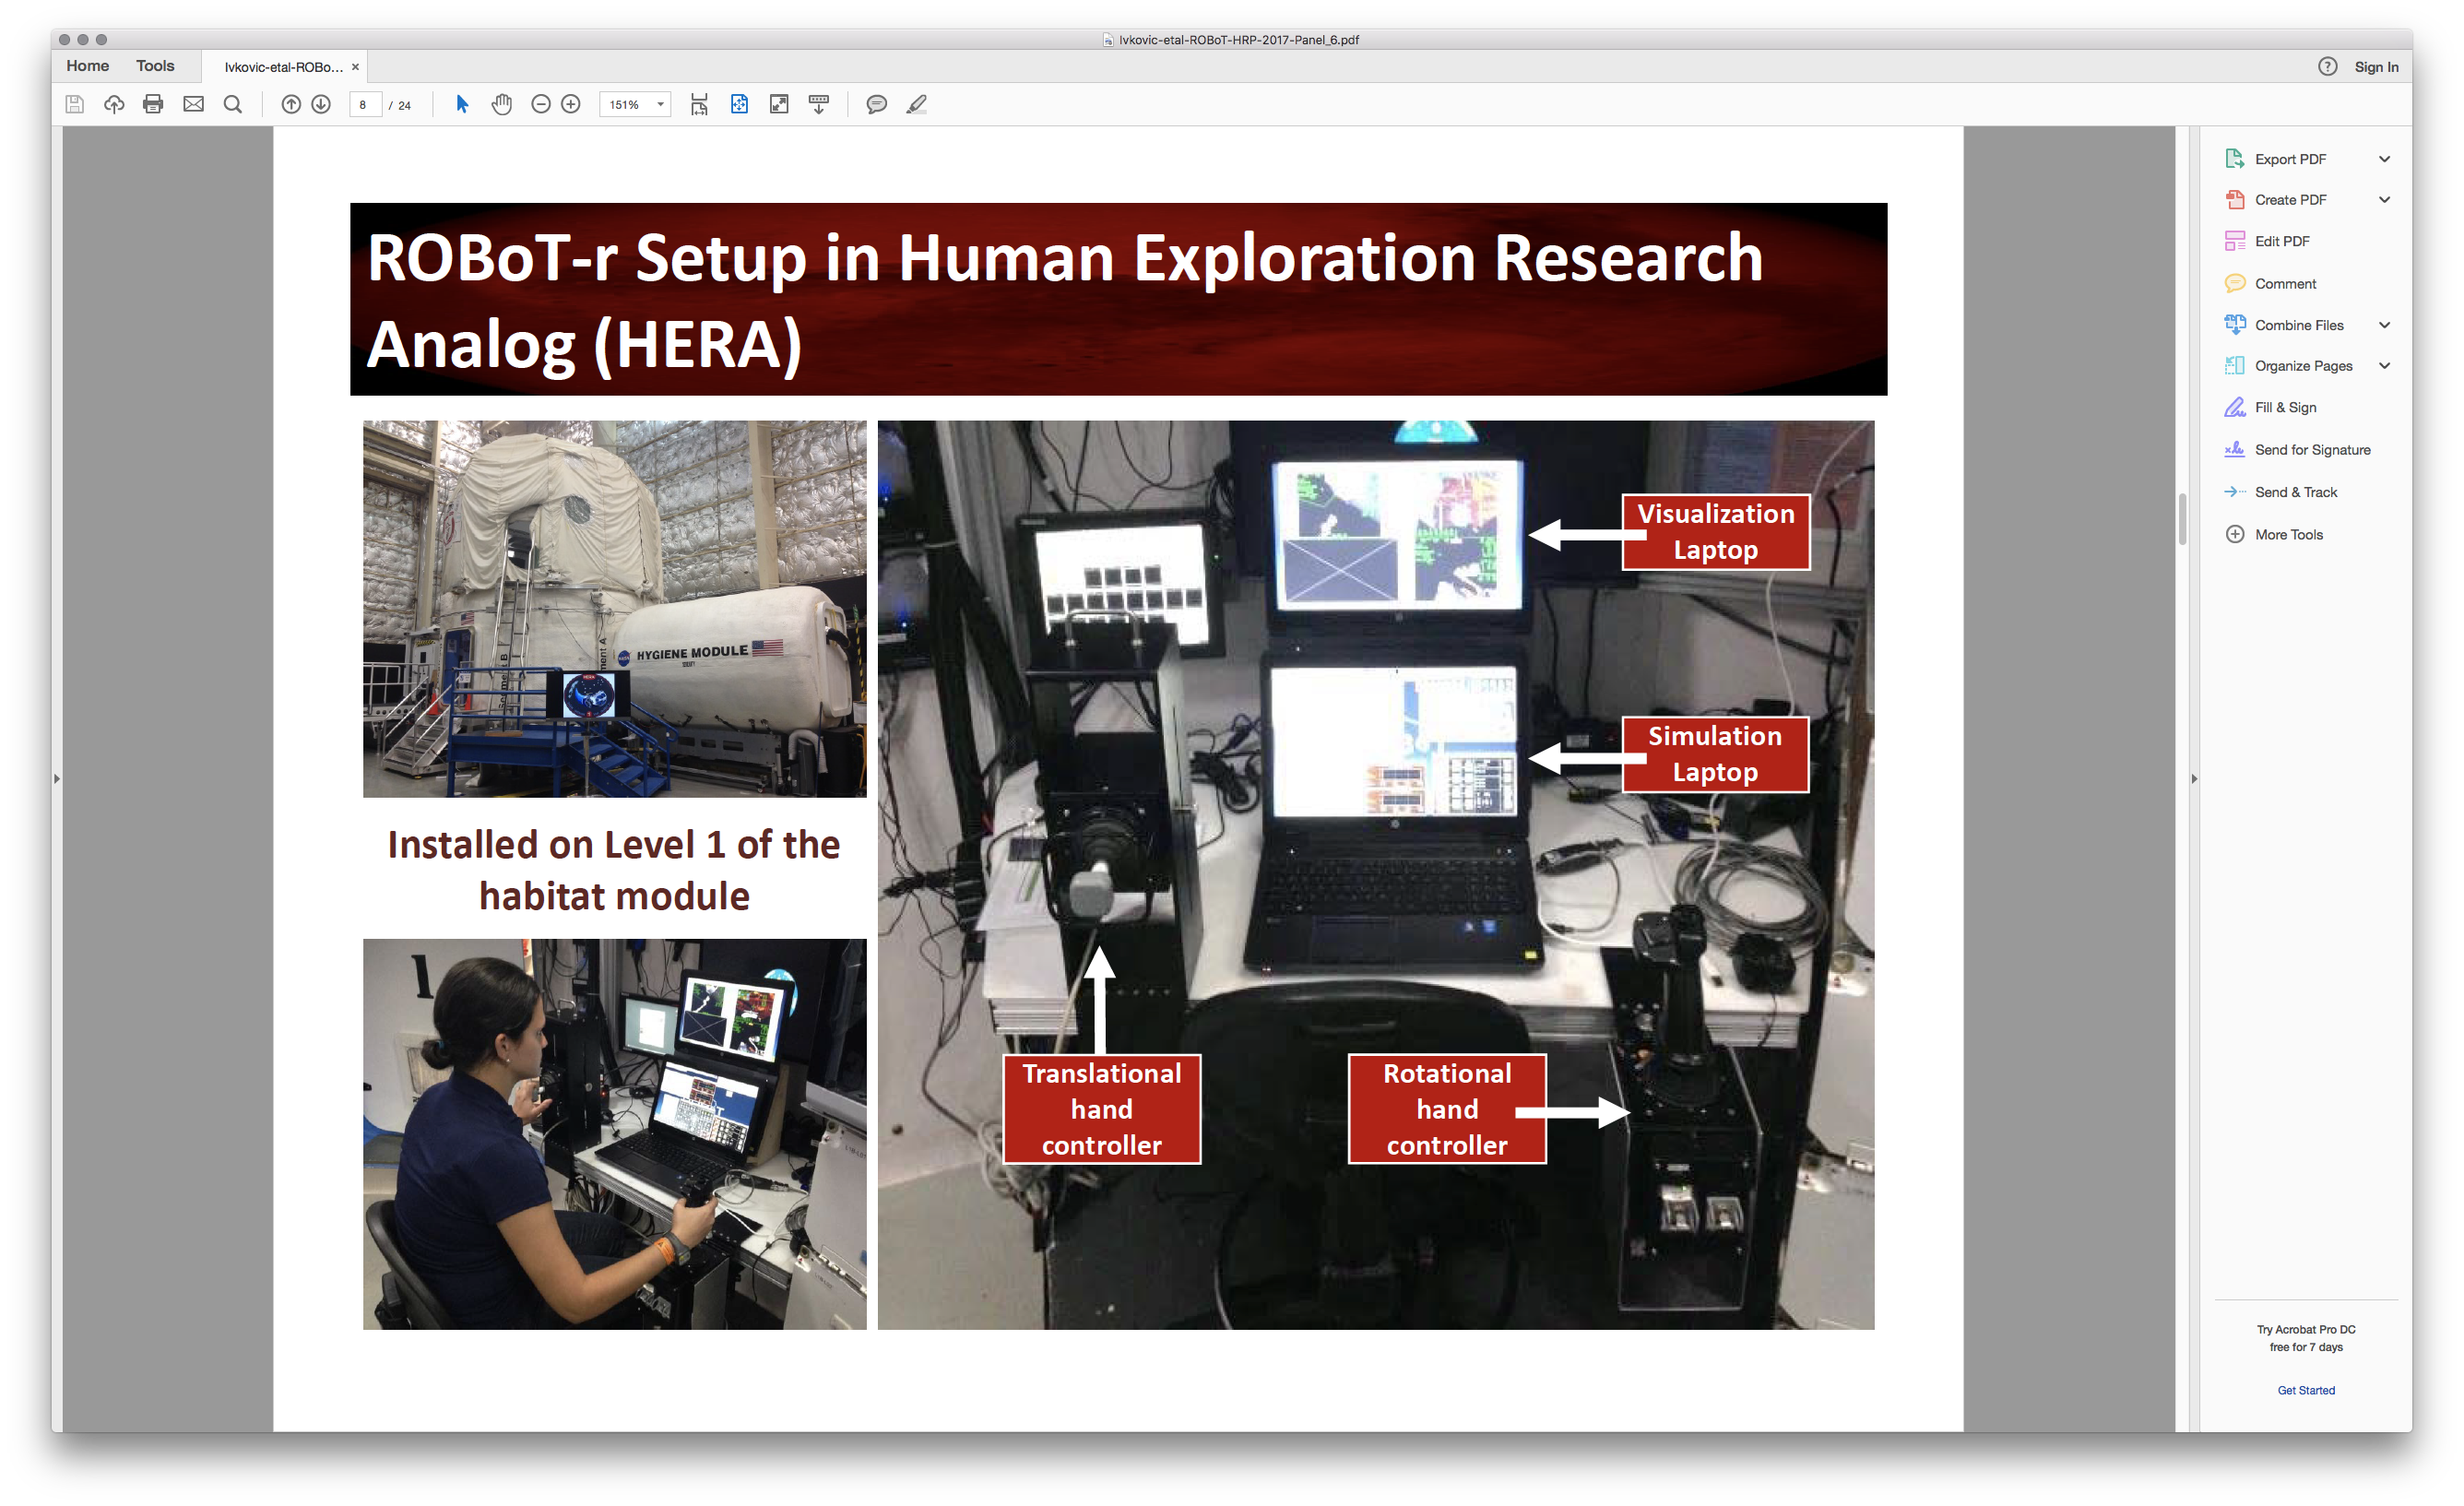
\includegraphics[trim={13cm 5cm 22cm 15.5cm},clip,width=\linewidth]{img/Screen Shot 2018-07-26 at 1.43.16 PM.png}
        \caption{The Robotic Onboard Trainer (ROBoT) station set up in the NASA HERA Analog.}
        % \label{}
    \end{center}
\end{figure}

\begin{figure}[tb!]
    \begin{center}
        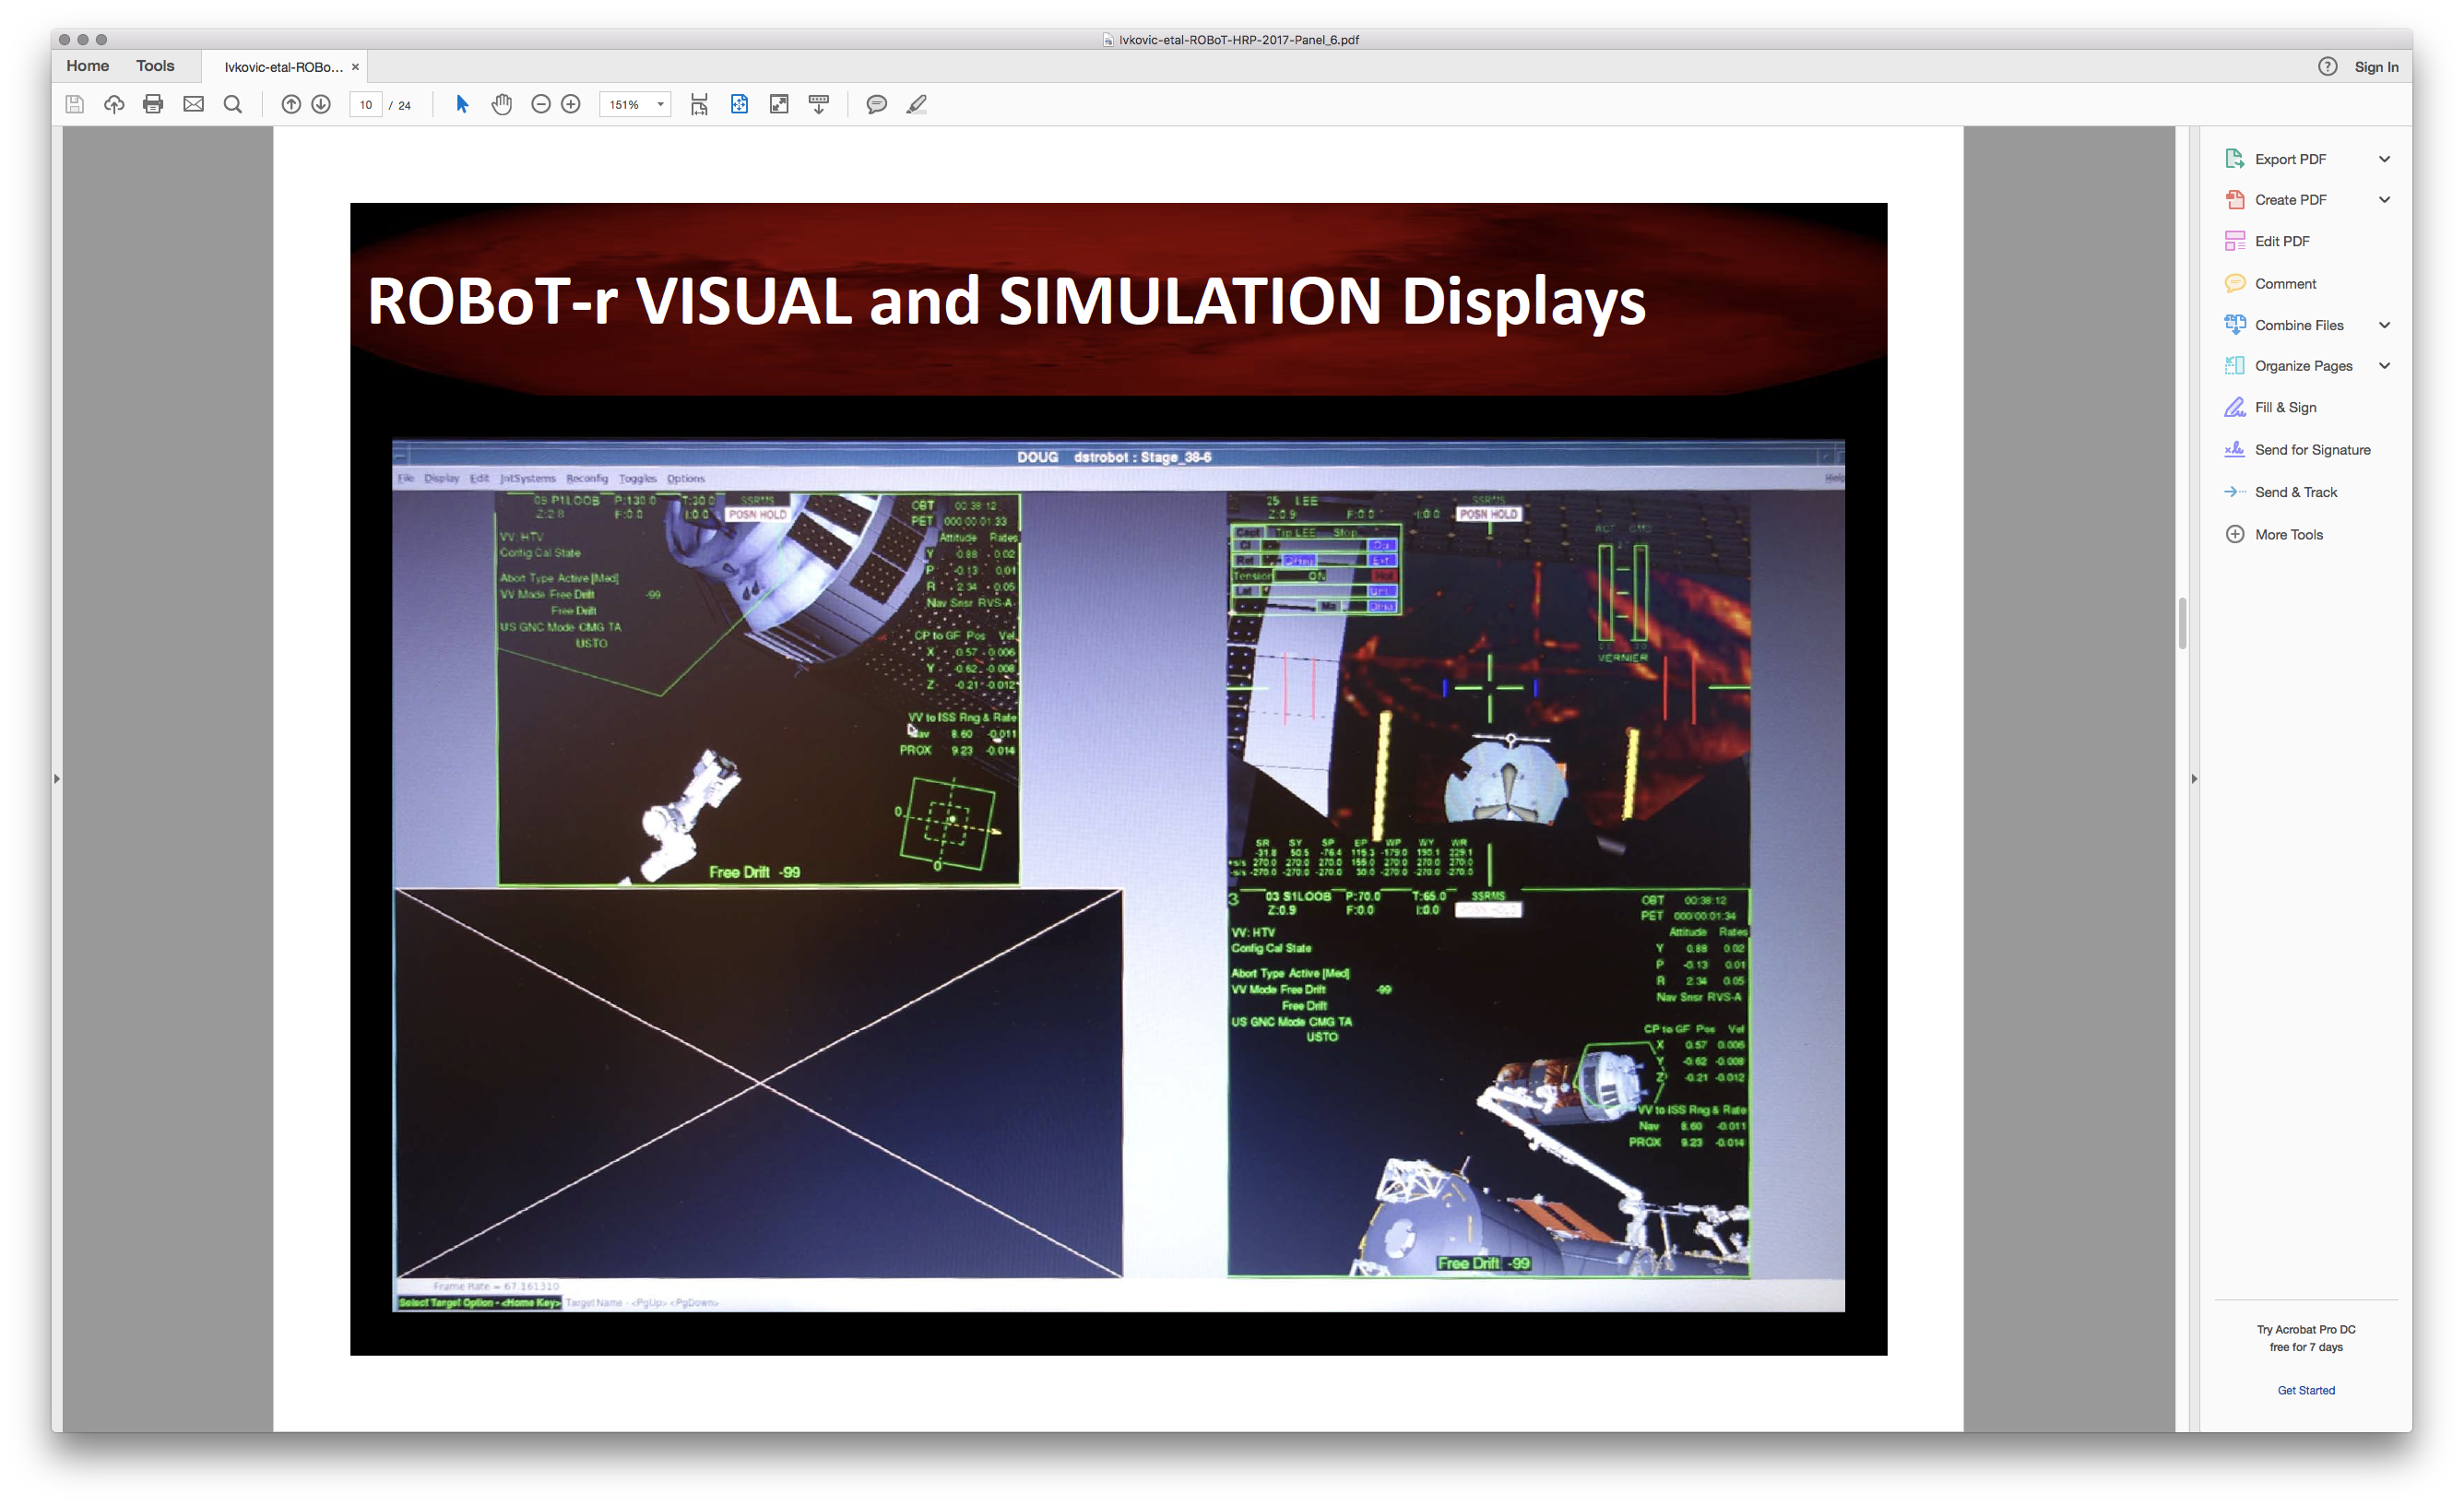
\includegraphics[trim={13cm 5cm 22cm 15.5cm},clip,width=\linewidth]{img/Screen Shot 2018-07-26 at 1.43.02 PM.png}
        \caption{ROBoT visualization laptop, showing four camera views.}
        % \label{}
    \end{center}
\end{figure}

\begin{figure}[tb!]
    \begin{center}
        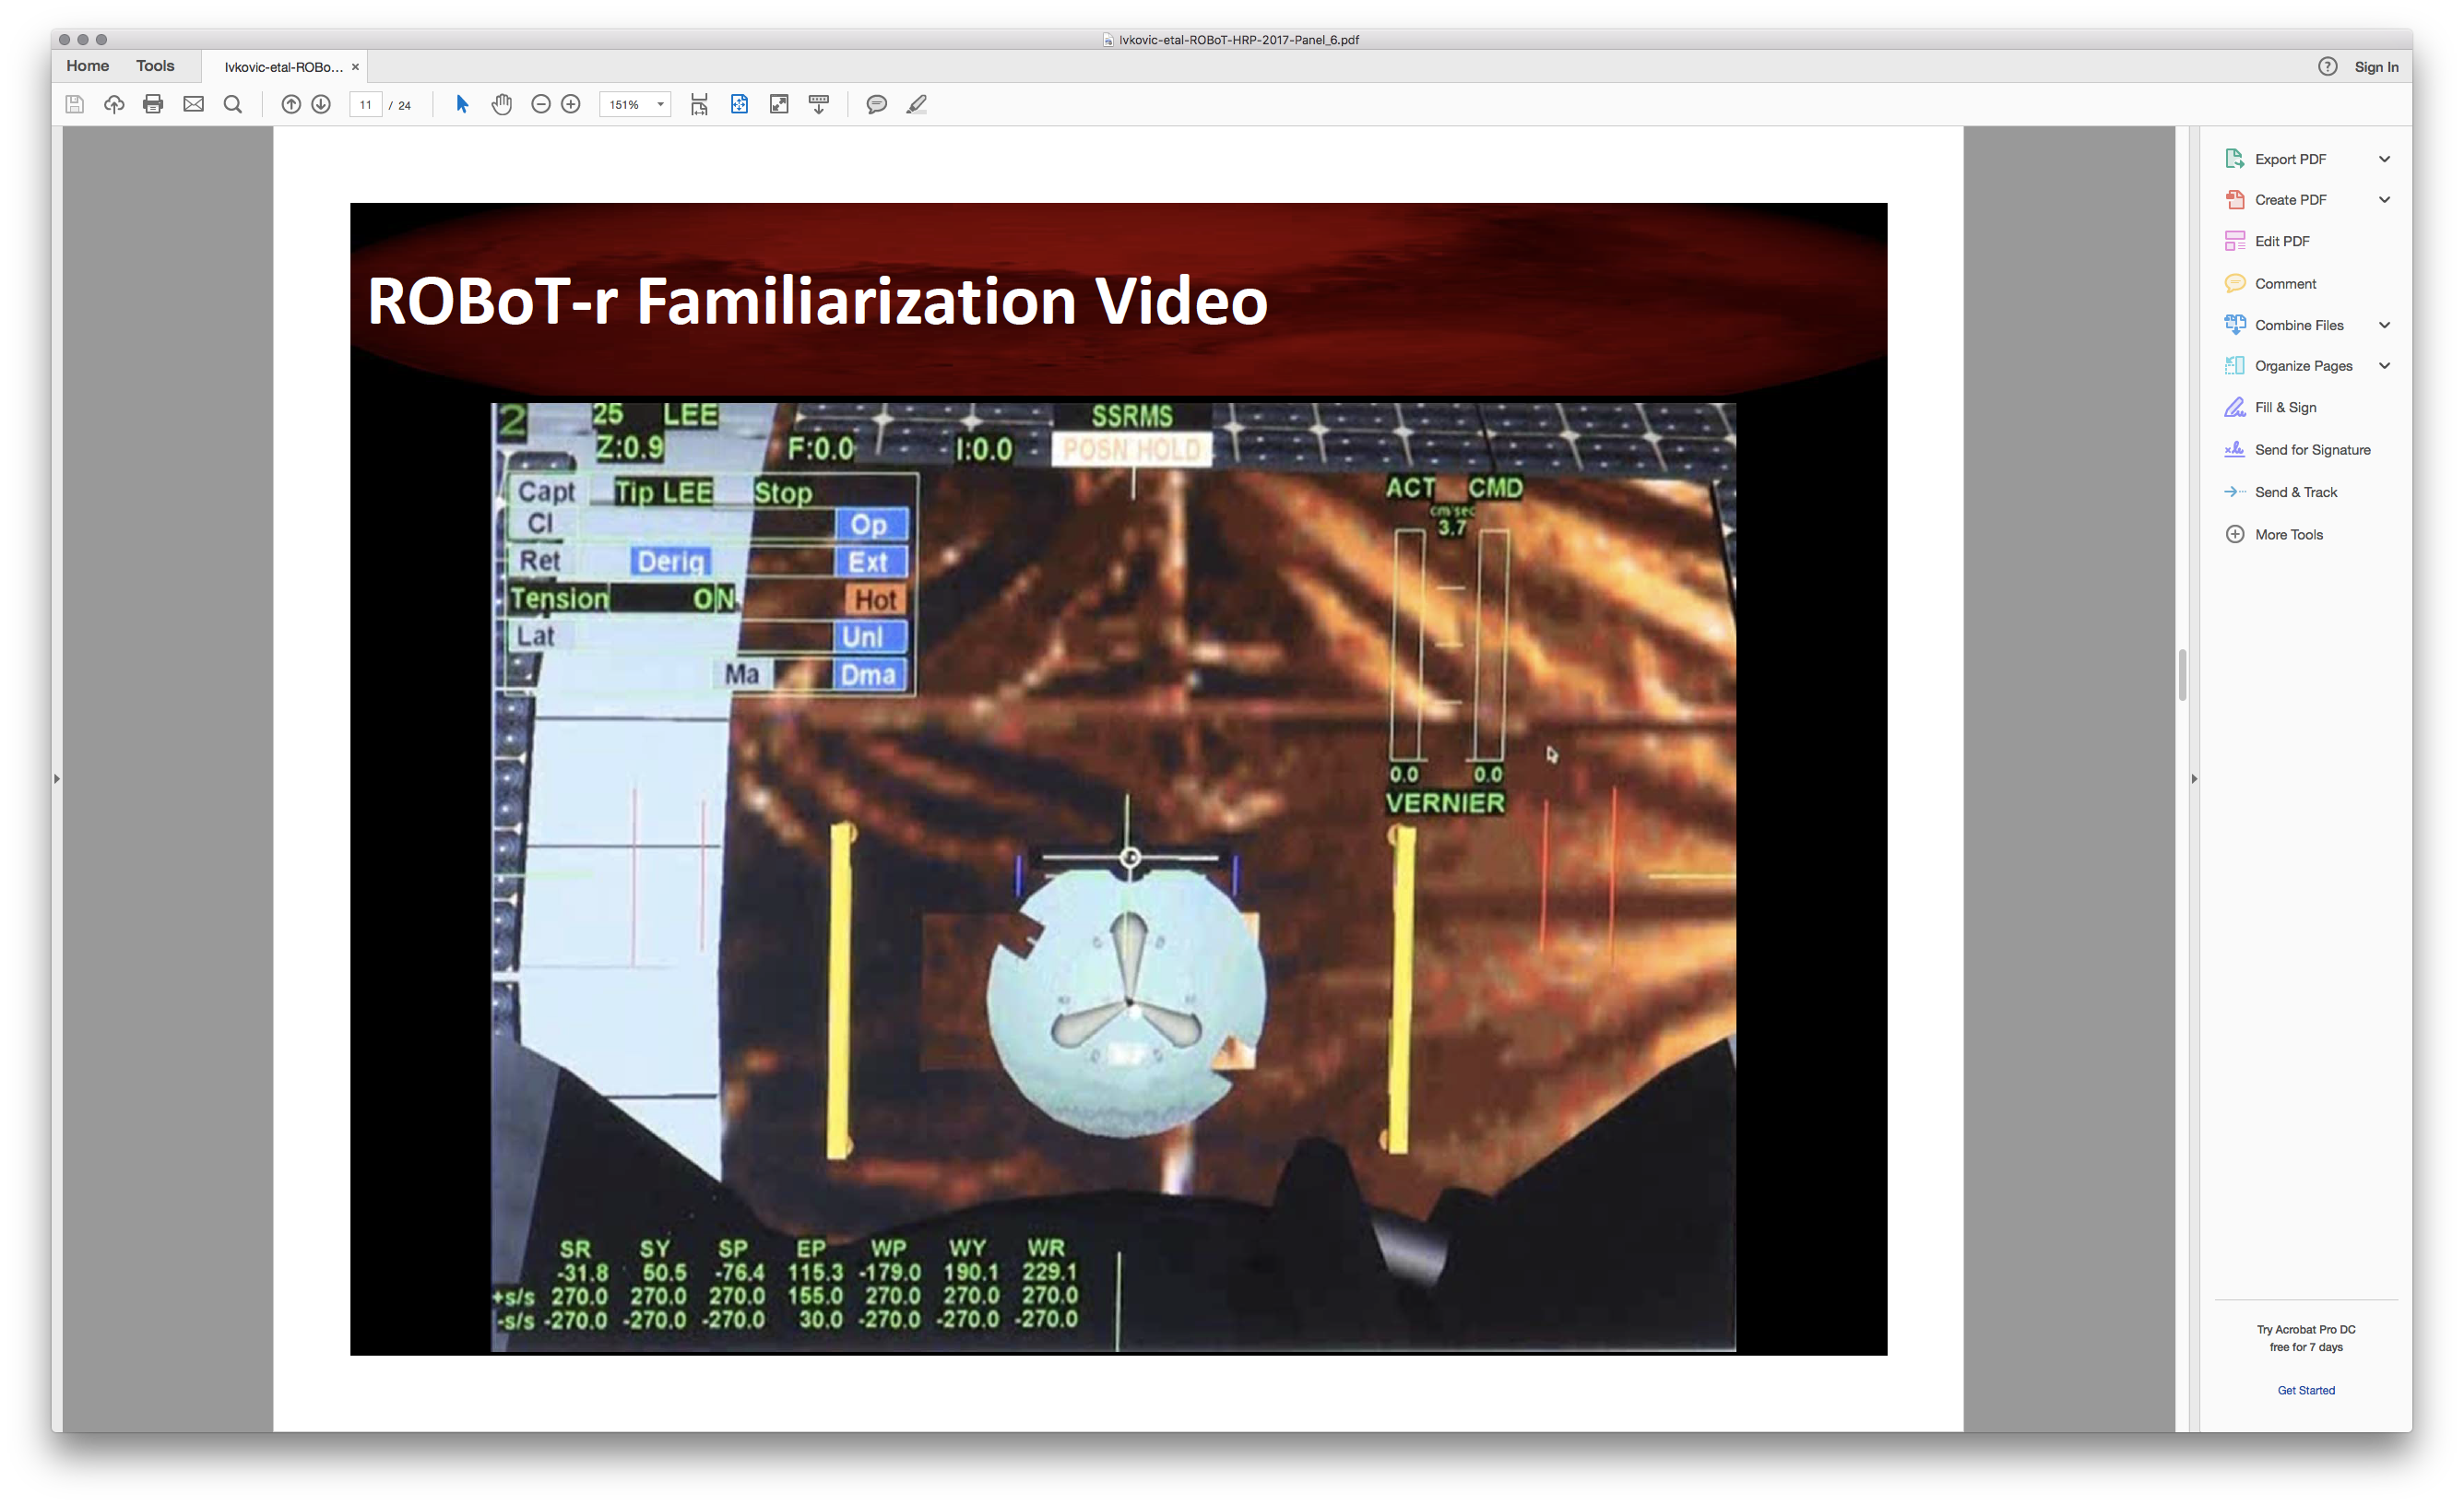
\includegraphics[trim={13cm 5cm 22cm 15.5cm},clip,width=\linewidth]{img/Screen Shot 2018-07-26 at 1.43.05 PM.png}
        \caption{The camera attached to the end effector of the robotic arm, showing the grapple fixture.}
        % \label{}
    \end{center}
\end{figure}

% \begin{figure}[tb!]
%     \begin{center}
%         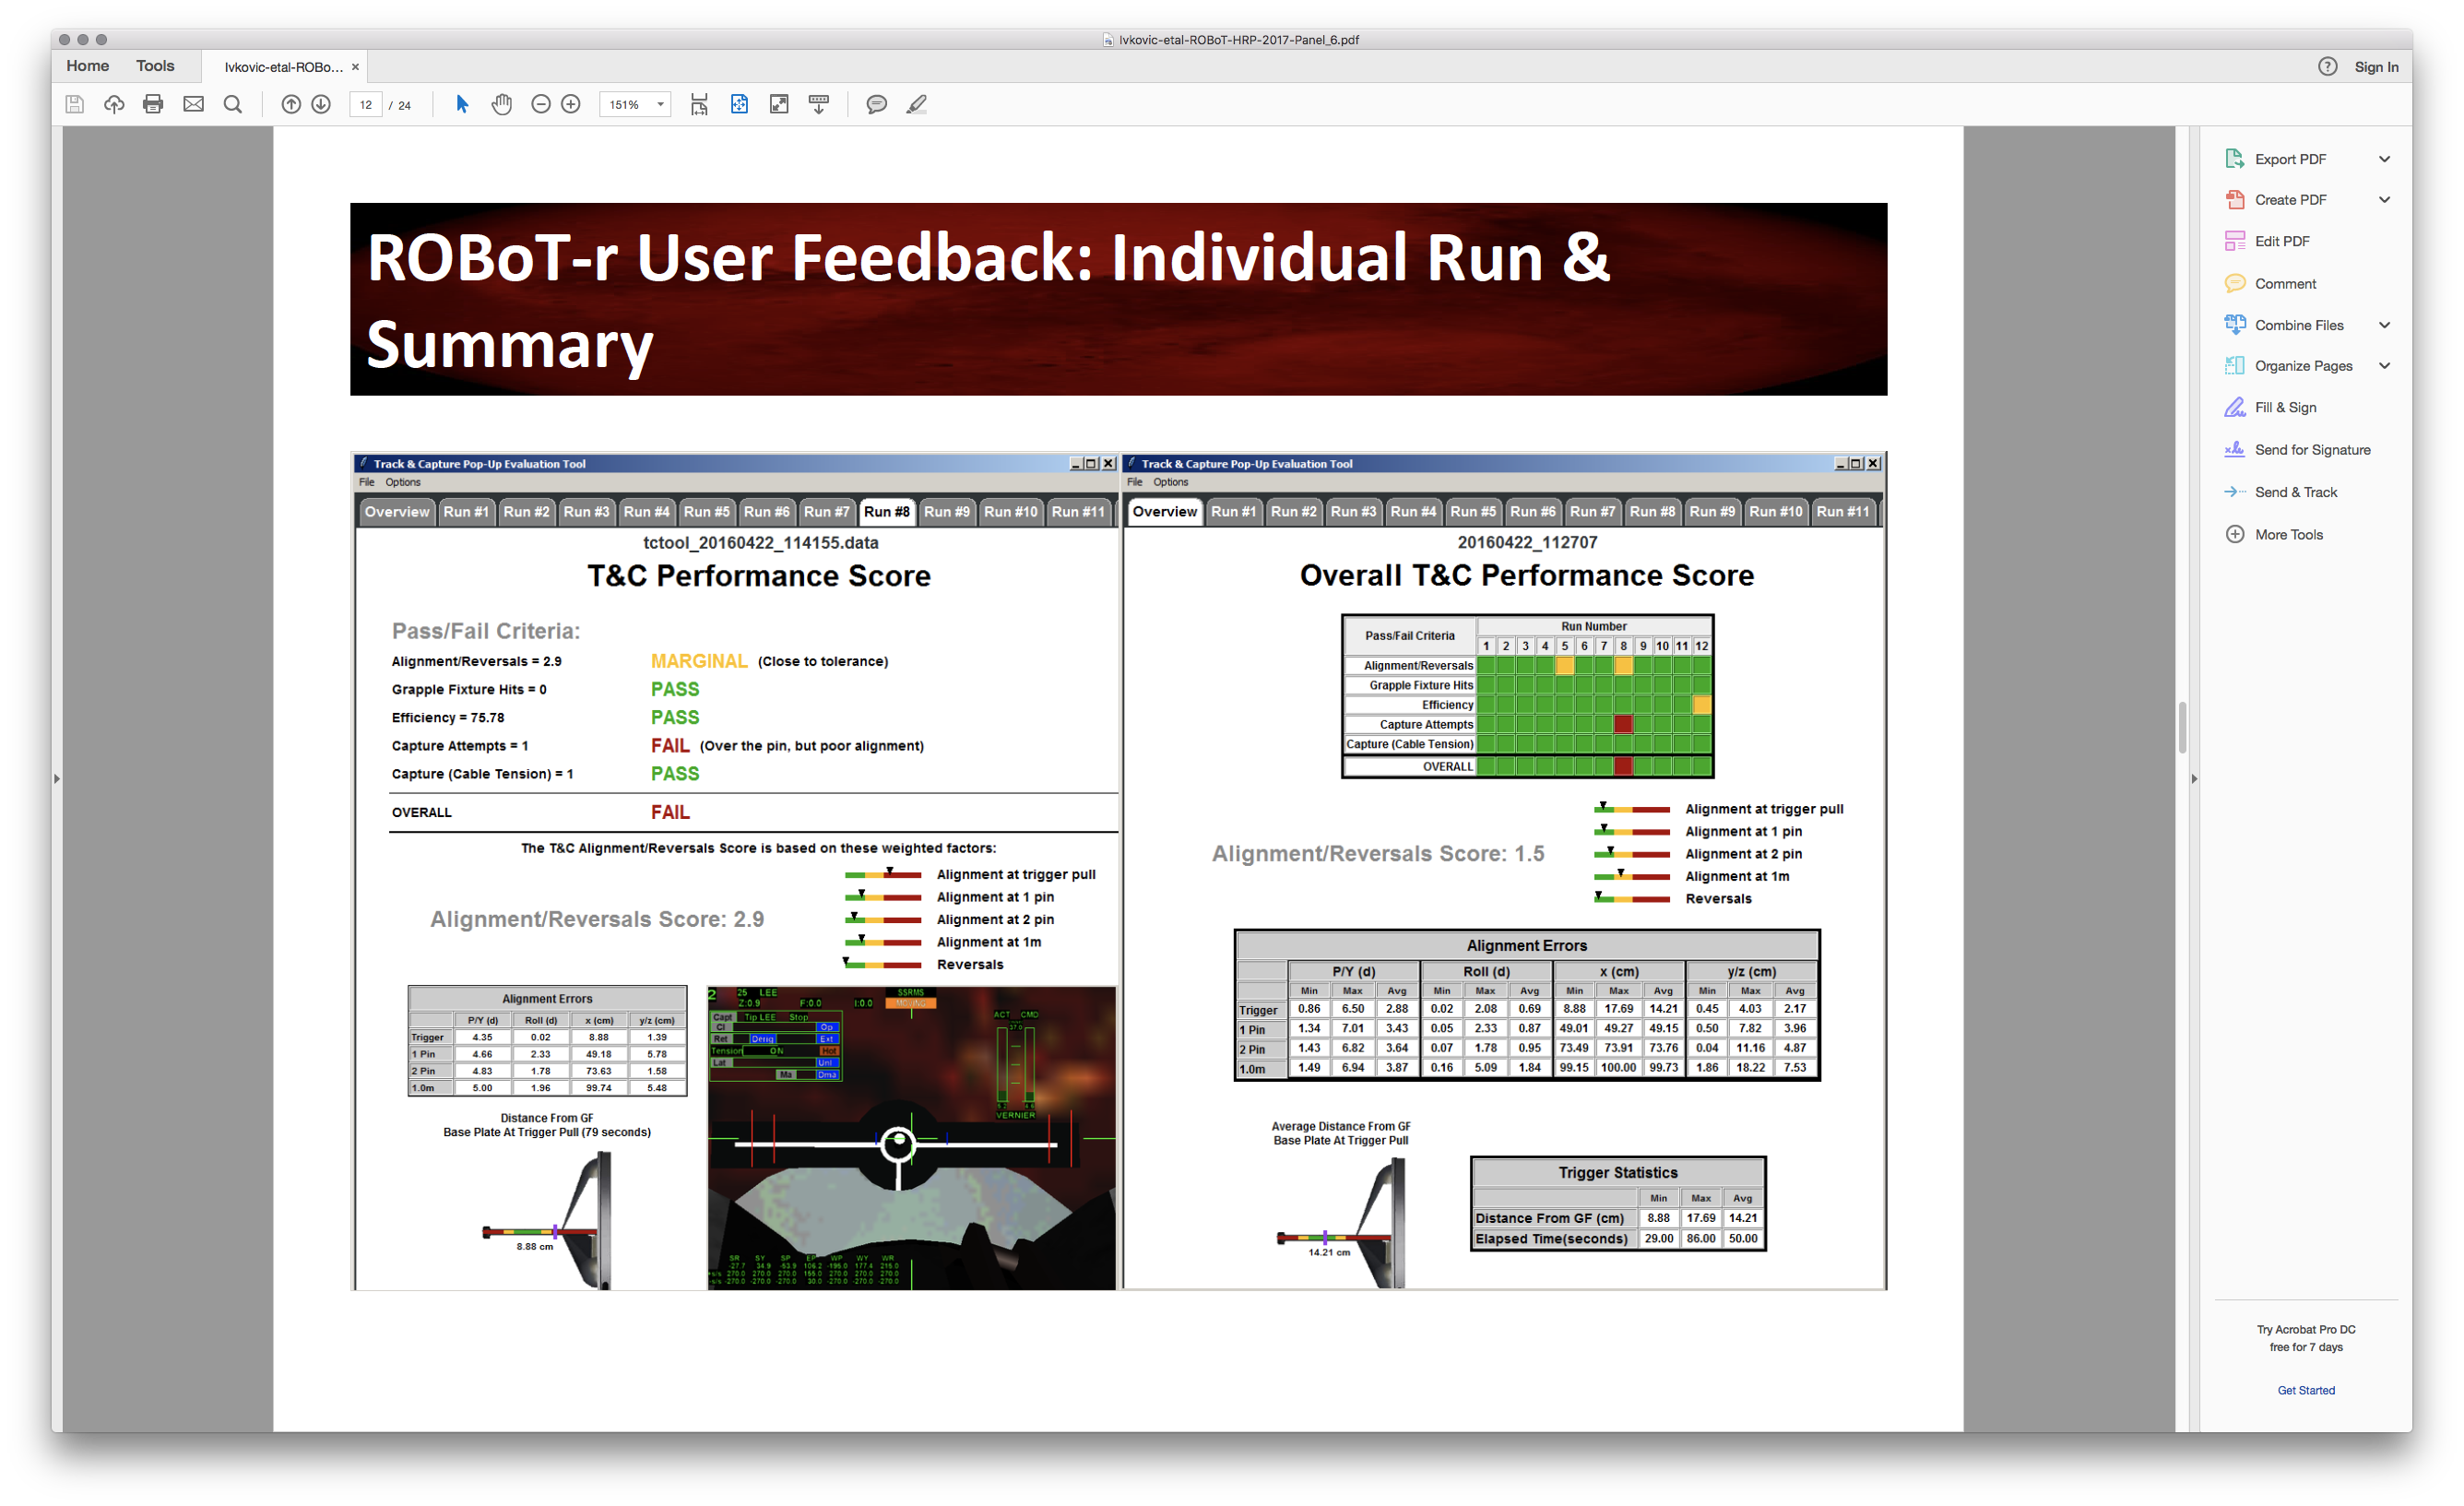
\includegraphics[trim={13cm 5cm 22cm 15.5cm},clip,width=\linewidth]{img/Screen Shot 2018-07-26 at 1.43.07 PM.png}
%         \caption{Example performance score report shown to the user after each trial.}
%         % \label{}
%     \end{center}
% \end{figure}

% \begin{figure}[tb!]
%     \begin{center}
%         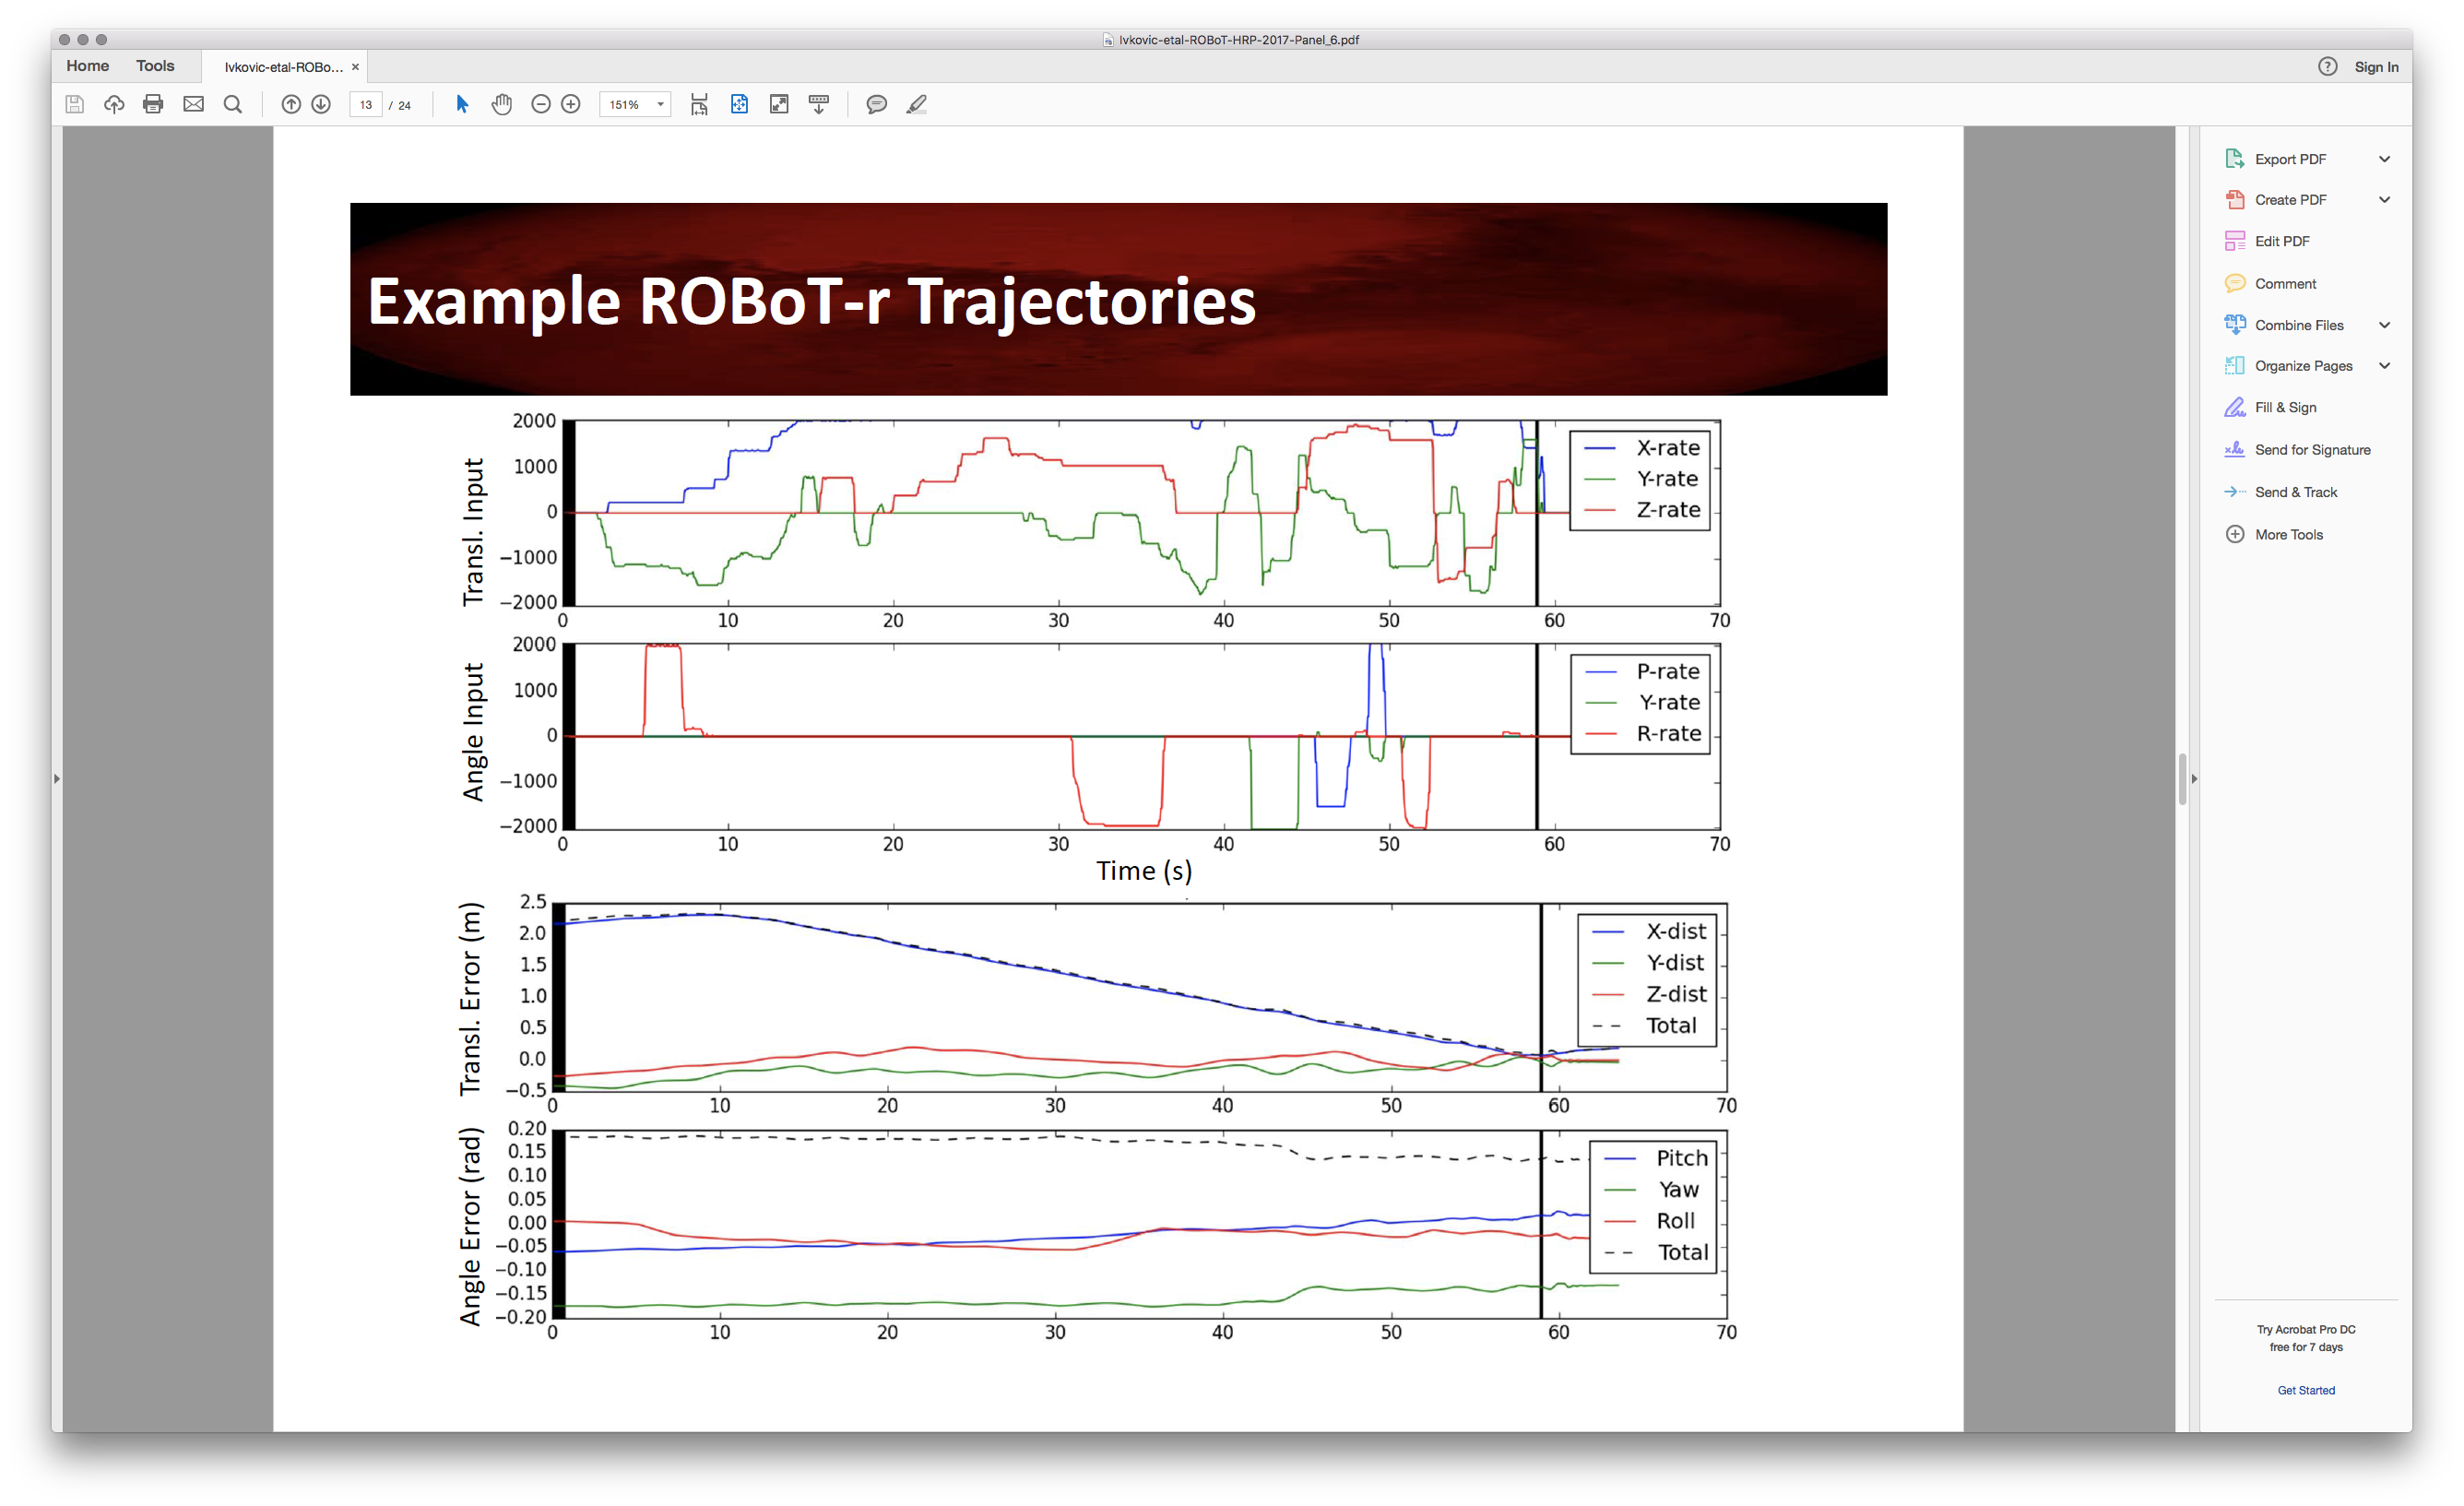
\includegraphics[trim={13cm 5cm 22cm 15.5cm},clip,width=\linewidth]{img/Screen Shot 2018-07-26 at 1.43.10 PM.png}
%         \caption{The hand controller inputs and position and angular errors are also logged throughout the trial.}
%         % \label{}
%     \end{center}
% \end{figure}


\subsection{Model Extension}
The Model will extend Professor Hess’ structural model of the human pilot to include the effects of concurrent bandwidth feedback.
The outputs of this model will be compared to the results of Experiment One and Two.

\subsection{Timeline}

\begin{figure}[h!]
    \begin{center}
        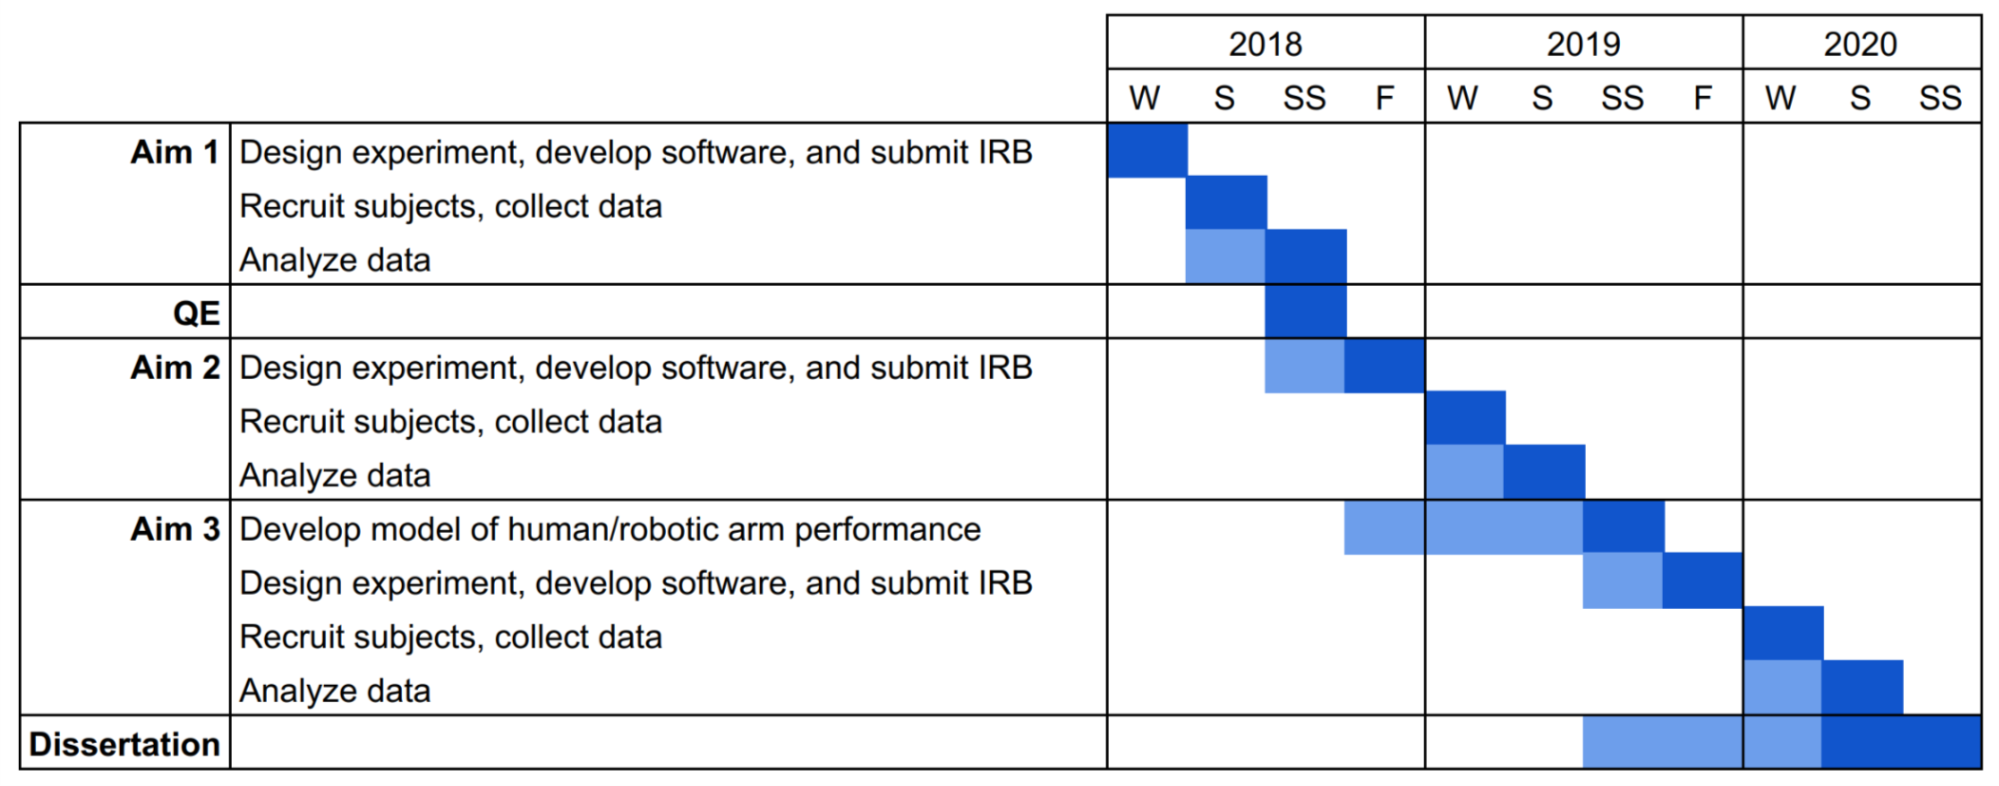
\includegraphics[width=\linewidth]{img/image1.png}
        % \caption{}
        % \label{}
    \end{center}
\end{figure}

\section{Conclusions}
Improving performance leads to smaller chance of critical errors in high risk environments in a near future with a larger number of potentially less trained actors in space

\bibliographystyle{ieeetr}
\bibliography{MyCollection}

\end{document}
